\documentclass{article}
\usepackage[english]{babel}

% Set page size and margins
% Replace `letterpaper' with `a4paper' for UK/EU standard size
\usepackage[letterpaper,top=2cm,bottom=2cm,left=2cm,right=2cm,marginparwidth=1.75cm, ]{geometry}

% Useful packages
\usepackage{color}
\usepackage[dvipsnames]{xcolor}

\definecolor{plasmadarkgreen}{RGB}{44, 75, 78}
\definecolor{plasmagreen}{RGB}{69, 115, 105}
\definecolor{plasmalightgreen}{RGB}{89, 184, 184}

\usepackage{esint}
\usepackage{amssymb}
\usepackage{relsize}
\usepackage{graphicx}
\usepackage[colorlinks=true, allcolors=plasmagreen]{hyperref}
\usepackage{setspace}
\usepackage{float}      % for putting [H] condition to figures etc.
\usepackage{fancyhdr}   % for page style 
\usepackage{minted}  % for python code
\usepackage{subfiles}
\usepackage[font={small}]{caption} 
\usemintedstyle{emacs}
\usepackage{titlesec}
\usepackage{tikz}
\usetikzlibrary{arrows.meta, positioning}
\usepackage[most]{tcolorbox}

\usepackage[ISO]{diffcoeff}[=v4]
\usepackage{mathtools}
% % load after mathtools (which loads amsmath)
\usepackage{amsthm}

\graphicspath{ {./figures/} }

% Define section and subsection colors
\titleformat{\section}
{\color{plasmadarkgreen}\normalfont\Large\bfseries}
{\color{plasmadarkgreen}\thesection}{1em}{}

\titleformat{\subsection}
{\color{plasmalightgreen}\normalfont\Large\bfseries}
{\color{plasmalightgreen}\thesubsection}{1em}{}

\titleformat{\subsubsection}
{\color{plasmagreen}\normalfont\Large\bfseries}
{\color{plasmagreen}\thesubsubsection}{1em}{}

\addto\captionsenglish{\renewcommand{\contentsname}{\bfseries{Table of Contents}}}


% Shortcuts

% Please use the following shortcuts when you update a theory section or add a new one for consistency and 
% clarity of the document for future editing.

\newcommand{\todo}[1]{{\color{red}{#1}}}

\newcommand{\jac}{\sqrt{g}}
\newcommand{\B}{\mathbf{B}}
\newcommand{\J}{\mathbf{J}}
\newcommand{\e}{\mathbf{e}}

\newcommand{\dFluxRho}{\cfrac{\partial \psi_{T}}{\partial \rho}}

\newcommand{\dRr}{\cfrac{\partial R}{\partial \rho}}
\newcommand{\dRt}{\cfrac{\partial R}{\partial \theta}}
\newcommand{\dRz}{\cfrac{\partial R}{\partial \zeta}}

\newcommand{\dZr}{\cfrac{\partial Z}{\partial \rho}}
\newcommand{\dZt}{\cfrac{\partial Z}{\partial \theta}}
\newcommand{\dZz}{\cfrac{\partial Z}{\partial \zeta}}

\newcommand{\dLr}{\cfrac{\partial \lambda}{\partial \rho}}
\newcommand{\dLt}{\cfrac{\partial \lambda}{\partial \theta}}
\newcommand{\dLz}{\cfrac{\partial \lambda}{\partial \zeta}}

\newcommand{\Brho}{(B^\theta \e_\theta + B^\zeta \e_\zeta) \cdot \e_\rho}
\newcommand{\Btheta}{(B^\theta \e_\theta + B^\zeta \e_\zeta) \cdot \e_\theta}
\newcommand{\Bzeta}{(B^\theta \e_\theta + B^\zeta \e_\zeta) \cdot \e_\zeta}

\newcommand{\Bvector}{ \cfrac{1}{2\pi\jac}\dFluxRho\begin{bmatrix}
        \left(\iota - \dLz\right)\e_{\theta} + \left(1 + \dLt\right) \e_\zeta
    \end{bmatrix}
}

\newcommand{\Bvectoreval}{ \cfrac{1}{2\pi\jac}\dFluxRho\begin{bmatrix}
        \left(\iota - \dLz\right)\e_{\theta}|_{\rho,\zeta} + \left(1 + \dLt\right) \e_\zeta|_{\rho,\theta}
    \end{bmatrix}
}

\newcommand{\BsupT}{\cfrac{1}{2\pi\jac}\dFluxRho\left(\iota - \dLz\right)}
\newcommand{\BsupZ}{\cfrac{1}{2\pi\jac}\dFluxRho\left(1 + \dLt\right)}
\newcommand{\Jacobian}{R \left( \dRr  \dZt + \dRt  \dZr \right)}



% --- common math notation ---
\DeclarePairedDelimiter{\abs}{\lvert}{\rvert}
\DeclarePairedDelimiter{\norm}{\lVert}{\rVert}
\DeclarePairedDelimiter{\ceil}{\lceil}{\rceil}
\DeclarePairedDelimiter{\floor}{\lfloor}{\rfloor}
\DeclarePairedDelimiter{\group}{\lparen}{\rparen}
\DeclarePairedDelimiter{\groupbrack}{\lbrack}{\rbrack}

% see mathtools package section 3.6 for explanation of the below set command
% just to make sure it exists
\ProvideDocumentCommand{\given}{}{}
% can be useful to refer to this outside \set
\NewDocumentCommand{\setSymbol}{o}{
    \mathchoice{\:}{\:}{\,}{\,}\IfValueT{#1}{#1}\vert
    \allowbreak
    \mathchoice{\:}{\:}{\,}{\,}
    \mathopen{}}
\DeclarePairedDelimiterX{\set}[1]{\lbrace}{\rbrace}{%
    \RenewDocumentCommand{\given}{}{\setSymbol[\delimsize]}
    #1
}
% intervals
\DeclarePairedDelimiterX{\closeint}[2]{\lbrack}{\rbrack}{#1, #2}
\DeclarePairedDelimiterX{\openint}[2]{\lparen}{\rparen}{#1, #2}
\DeclarePairedDelimiterX{\clopenint}[2]{\lbrack}{\rparen}{#1, #2}
\DeclarePairedDelimiterX{\openclint}[2]{\lparen}{\rbrack}{#1, #2}
% inner product
\DeclarePairedDelimiterX{\innerp}[2]{\langle}{\rangle}{#1, #2}
% sign function
\DeclareMathOperator{\sign}{sign}
% natural numbers from 1 to given argument
\NewDocumentCommand{\nats}{m}{\symbb{N} \cap \closeint{1}{#1}}
% integers from 0 to given argument
\NewDocumentCommand{\ints}{m}{\symbb{Z} \cap \closeint{0}{#1}}

% --- linear algebra ---
% transpose
\NewDocumentCommand{\trans}{m}{{#1}^{\mathsf{T}}}
% Hermitian (conjugate) transpose
\NewDocumentCommand{\herm}{m}{{#1}^{\mathsf{H}}}
% image of argument (subset of codomain)
\DeclareMathOperator{\image}{image}
% rank of matrix
\DeclareMathOperator{\rank}{rank}
% dimension of kernel
\DeclareMathOperator{\nullity}{nullity}
% % bold vectors
% \AtBeginDocument{\RenewDocumentCommand{\vec}{m}{\mathbf{#1}}}
\DeclarePairedDelimiter{\mean}{\langle}{\rangle}

\newtcbox{\class}[1][]{on line,
    colback=plasmalightgreen,
    coltext=white,
    boxrule=0pt,
    arc=4pt, % Controls the roundness of corners
    boxsep=1pt,
    left=2pt,
    right=2pt,
    top=1pt,
    bottom=1pt,
    #1}
    
\newtcbox{\obj}[1][]{on line,
    colback=plasmagreen,
    coltext=white,
    boxrule=0pt,
    arc=4pt, % Controls the roundness of corners
    boxsep=1pt,
    left=2pt,
    right=2pt,
    top=1pt,
    bottom=1pt,
    #1}

\newtcbox{\opt}[1][]{on line,
    colback=plasmadarkgreen,
    coltext=white,
    boxrule=0pt,
    arc=4pt, % Controls the roundness of corners
    boxsep=1pt,
    left=2pt,
    right=2pt,
    top=1pt,
    bottom=1pt,
    #1}
\newcommand{\function}[1]{{\color{blue}{#1}}}
\newcommand{\attribute}[1]{{\color{red}{#1}}}
\newcommand{\dx}{\Delta x}
\newcommand{\dc}{\Delta c}


\title{Introduction to DESC and Stellarators}
\author{Yigit Gunsur Elmacioglu. Kaya Unalmis}

\begin{document}
\onehalfspacing
\maketitle

\pagebreak
{\footnotesize \tableofcontents
                \listoftables
                \listoffigures
} 

\pagebreak
\pagenumbering{arabic}
\pagestyle{fancy}
\fancyhf{}
\fancyhead[L]{\textcolor{plasmalightgreen}{\rightmark}}  % Section in blue on the left
\fancyhead[R]{\textcolor{plasmadarkgreen}{\leftmark}}   % Chapter in red on the right (for books or report class)
\fancyfoot[R]{\color{plasmagreen}{\small{Princeton University - Plasma Control Group}}}
\let\oldheadrule\headrule% Copy \headrule into \oldheadrule
\renewcommand{\headrule}{\color{plasmagreen}\oldheadrule}% Add colour to \headrule
\renewcommand{\headrulewidth}{0.5pt}

% ======================================================================


\section{Introduction}

This document is for getting started with the basic maths used in Stellarators, more specifically the ones used in 3D MHD equilibrium code DESC. It will serve as a cheat sheet for the future. In preparation of this document, the book "An Introduction to Stellarators" by Imbert Gerard et al. is heavily used \cite{imbert-gerard_introduction_nodate}.


% ======================================================================


\section{Basis Functions}

\subfile{sections/basis/fourier-series.tex}
\pagebreak
\subfile{sections/basis/zernike-polynomials.tex}
\pagebreak
\subfile{sections/basis/fourier-zernike.tex}
\subfile{sections/basis/stell-sym.tex}


% ======================================================================


\pagebreak
\section{Coordinates}

Magnetic confinement machines have the shape of torus (or donut). Instead of using cartesian coordinate system which has straight lines as axis, due to the curved shaped of the torus, we can use curvilinear coordinates. For example, any function inside this geometry can be defined in terms of cylindrical coordinates with R (radial part), $\phi$ (toroidal angle) and Z (height). However, as you can see from the right side of Figure \ref{coords}, there is a more convenient set of curvilinear coordinates that can define any point of this torus which is called flux coordinates. 

\begin{figure}[H]
    \centering
    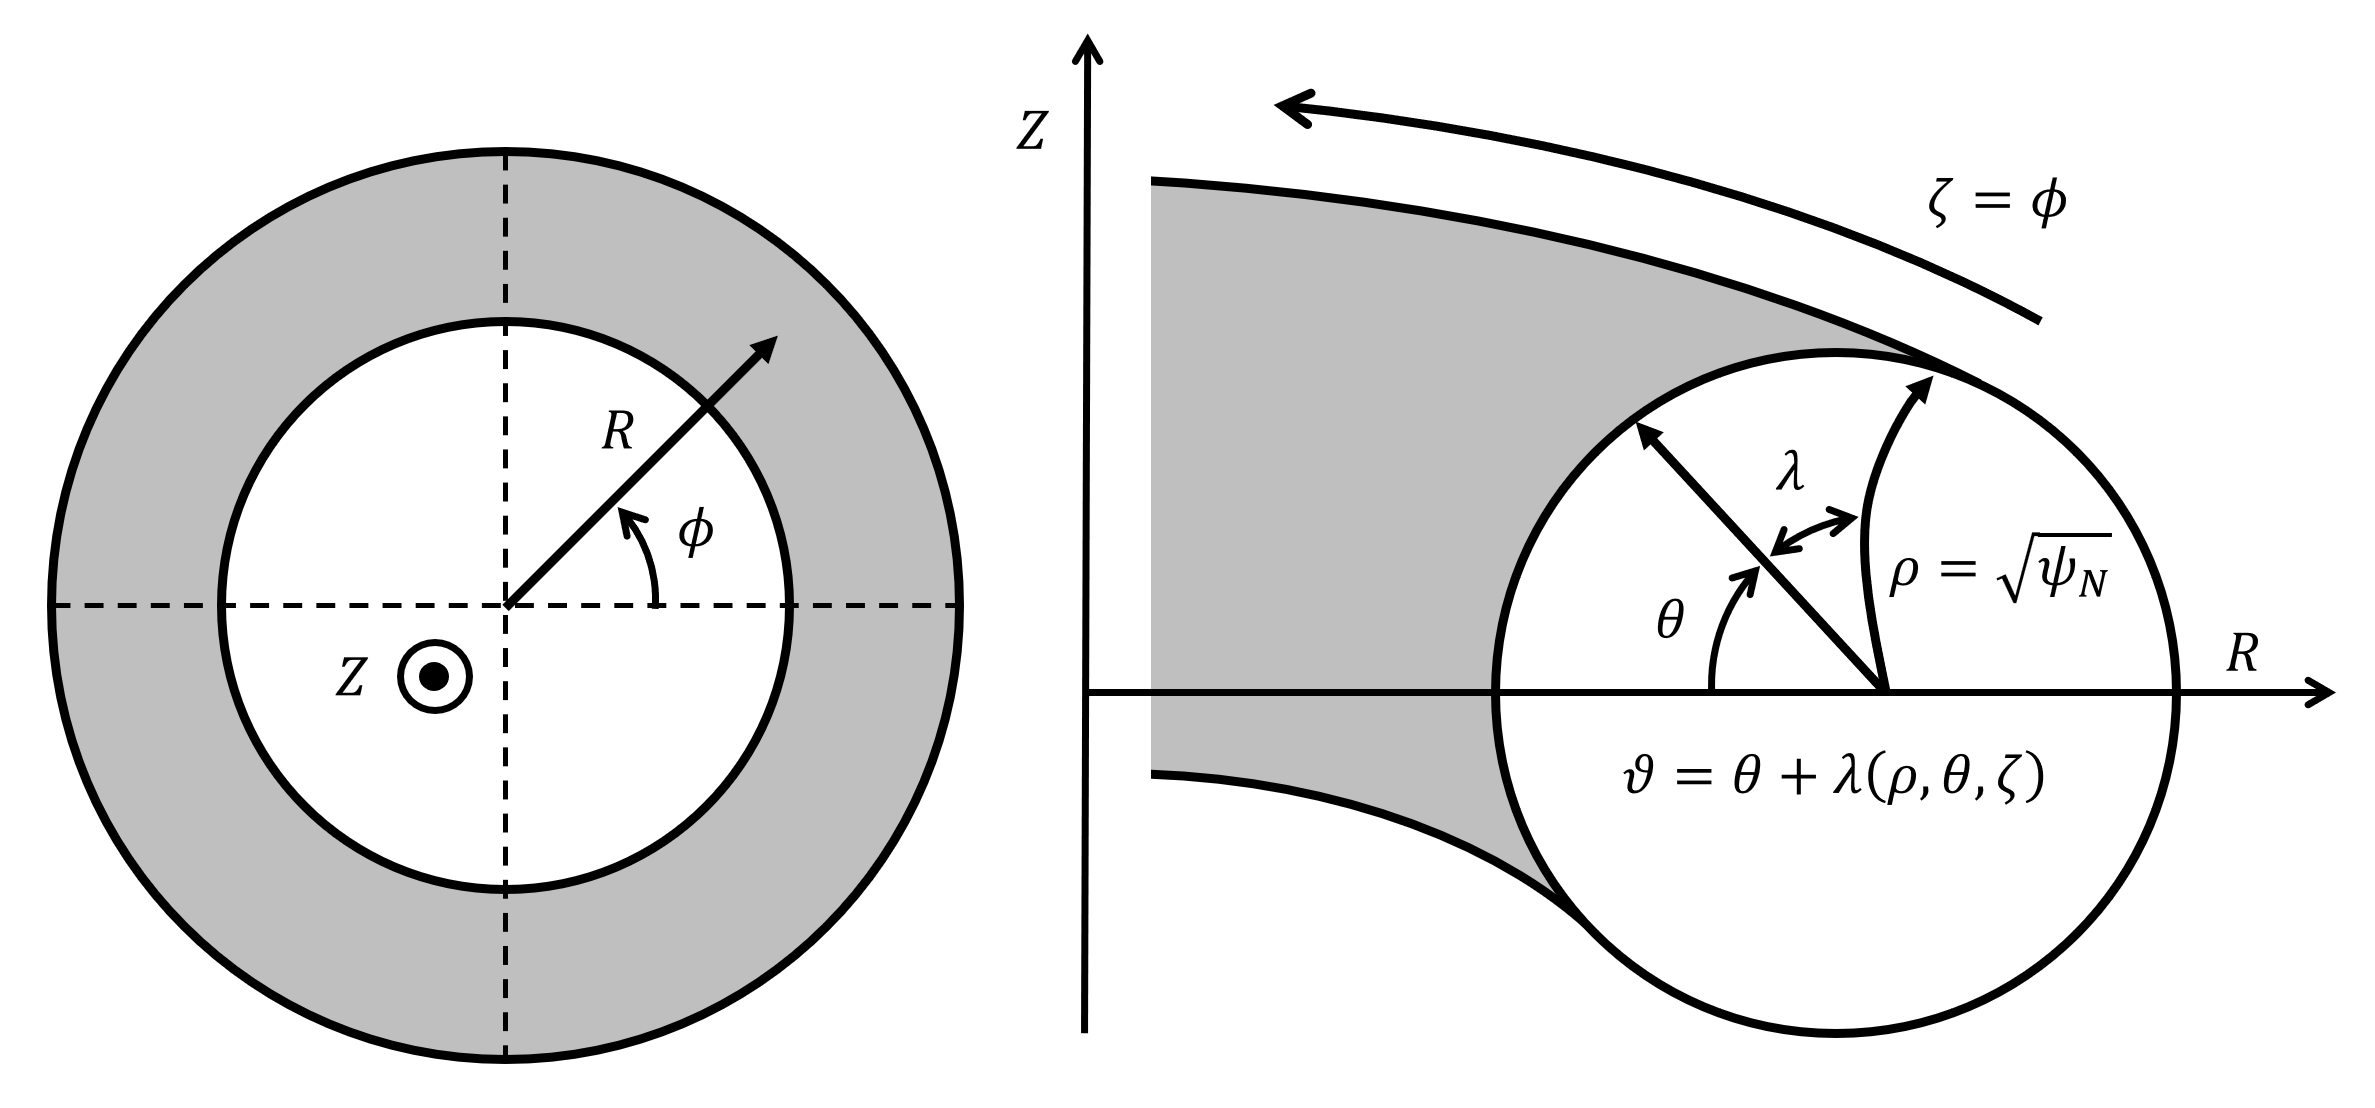
\includegraphics[width=0.8\textwidth]{coords.png}
    \caption{{\color{red}\textbf{Sketch a better figure for this}}}
    \label{coords}
\end{figure}

These coordinates are $\rho, \theta$ and $\zeta$. Here, $\zeta$ is exactly the same as $\phi$ in cylindrical coordinates. $\rho$ is similar to the radial coordinate of cylindrical coordinates but since we will try to find more intricate shapes rather than a bunch of circles, instead of defining it as the distance to the center, we will define it as a function of the flux and this will express the index of flux surface. Lastly, $\theta$ is the poloidal angle. 


\subfile{sections/coordinates/co-contravariant.tex}
\subfile{sections/coordinates/vector-operations.tex}
\subfile{sections/coordinates/desc-implementation.tex}


% ======================================================================


\pagebreak
\section{Fields}

\subfile{sections/fields/rotational-transform.tex}
\subfile{sections/fields/ideal-mhd.tex}
\subfile{sections/fields/rotational-transform-computation.tex}


% ======================================================================


\pagebreak
\section{Optimization}

\subfile{sections/optimization/optimization.tex}
\subfile{sections/optimization/proximal-projection.tex}


% ======================================================================

\pagebreak
\section{Profiling DESC}

\subfile{sections/profiling/profiling.tex}


% ======================================================================

\pagebreak
\section{Multi-Device Applications}

\subfile{sections/multi-device/mpi4jax.tex}


% ======================================================================

{\color{blue} \section{DON'T FORGET TO INCLUDE}
\begin{itemize}
    \item Better explain optimization
    \item Make better figure for coordinates
    \item Make a plot using Dario's script for covariant and contravariant basis vectors
\end{itemize}

}

\bibliographystyle{ieeetr}
\bibliography{bibtex}


% ======================================================================


\appendix
\section{Relation between Zernike Polynomials and Jacobi Polynomials}\label{appedix-2}
For the special case of $\beta=0$, $x=1-2\rho^2$ and $\alpha=m$, Jacobi Polynomials can be written using equation \ref{jacobi},
\begin{equation}
    P_{n}^{m, 0}(1-2\rho^2) = \sum_{s=0}^{n} (-1)^s\binom{n+m}{n-s} \binom{n}{s} \rho^{2s}(1-\rho^2)^{n-s} \label{eq_jac}
\end{equation}
Now, let's use binomial theorem to expand $(1-\rho^2)^{n-s}$,
\begin{equation}
    (1-\rho^2)^{n-s} = \sum_{k=0}^{n-s} (-1)^k \binom{n-s}{k} \rho^{2k}
\end{equation}
Substitute this in eq \ref{eq_jac},
\begin{equation}
    P_{n}^{m, 0}(1-2\rho^2) = \sum_{s=0}^{n} (-1)^s \binom{n}{s} \binom{n+m}{n-s}  \rho^{2s} \sum_{k=0}^{n-s} (-1)^k \binom{n-s}{k} \rho^{2k}
\end{equation}
Now, rearrange the terms,
\begin{equation}
    P_{n}^{m, 0}(1-2\rho^2) = \sum_{s=0}^{n}\sum_{k=0}^{n-s} (-1)^{(s+k)} \binom{n+m}{n-s} \binom{n}{s} \binom{n-s}{k} \rho^{2(s+k)}
\end{equation}
Substitute $j=s+k$, hence $k=j-s$ ,
\begin{align}
    P_{n}^{m, 0}(1-2\rho^2) &= \sum_{s=0}^{n}\sum_{j-s=0}^{j-s=n-s} (-1)^{j} \binom{n+m}{n-s} \binom{n}{s} \binom{n-s}{j-s}\rho^{2j}\\
    P_{n}^{m, 0}(1-2\rho^2) &= \sum_{s=0}^{n}\sum_{j=s}^{n} (-1)^{j} \binom{n+m}{n-s} \binom{n}{s} \binom{n-s}{j-s}\rho^{2j}  
\end{align}
Here, we can change the order of summation, it is better to use table to find new limits,
\[
\begin{array}{c|cccccc}
  & 0 & 1 & 2 & \cdots & n-1 & n \\
\hline
s = 0 & \times & \times & \times & \cdots & \times & \times \\
s = 1 &       & \times & \times & \cdots & \times & \times \\
s = 2 &       &       & \times & \cdots & \times & \times \\
\vdots &       &       &       & \ddots & \vdots & \vdots \\
s = n-1 &       &       &       &       & \times & \times \\
s = n &       &       &       &       &       & \times \\
\end{array}
\]
Each \(\times\) represents a valid pair \((s, j)\). This can be re-written in terms of summation over $j$ first, then $s$,
\[
\begin{array}{c|cccccc}
  & 0 & 1 & 2 & \cdots & n-1 & n \\
\hline
j = 0 & \times &       &       &       &       &       \\
j = 1 & \times & \times &       &       &       &       \\
j = 2 & \times & \times & \times &       &       &       \\
\vdots &       &       &       & \ddots &       &       \\
j = n-1 & \times & \times & \times & \cdots & \times &       \\
j = n & \times & \times & \times & \cdots & \times & \times \\
\end{array}
\]
Since the \((s, j)\) pairs are the same, the nested summation can be written as,
\begin{equation}
    P_{n}^{m, 0}(1-2\rho^2) = \sum_{j=0}^{n} \rho^{2j}   \sum_{s=0}^{j} (-1)^{j} \frac{(n+m)!}
    {(n-s)!(m+s)!}\frac{n!}{s!(n-s)!}\frac{(n-s)!}{(j-s)!(n-j)!}
\end{equation}
\begin{equation}
    P_{n}^{m, 0}(1-2\rho^2) = \sum_{j=0}^{n} \rho^{2j}   \sum_{s=0}^{j} (-1)^{j} \frac{(n+m)!}{(n-s)!(m+s)!} \frac{j!}{s!(j-s)!} \frac{n!}{j!(n-j)!} 
\end{equation}
\begin{equation}
    P_{n}^{m, 0}(1-2\rho^2) = \sum_{j=0}^{n} (-1)^{j} \binom{n}{j} \rho^{2j}   \sum_{s=0}^{j}  \binom{n+m}{n-s} \binom{j}{s}  \label{eq_jacobi2simplify}
\end{equation}
Now, we need to use a property of the binomial coefficients. Consider,
\begin{align}
    (1+x)^n =& \sum_{k=0}^{n} \binom{n}{k}x^k \\
    (1+x)^{n+m}(1+x)^j =&  \left(\sum_{k=0}^{n+m} \binom{n+m}{k}x^k\right) \left(\sum_{k=0}^{j} \binom{j}{k}x^k\right) = \left(\sum_{s=-m}^{n} \binom{n+m}{n-s}x^{n-s}\right) \left(\sum_{k=0}^{j} \binom{j}{k}x^k\right) \\
    (1+x)^{n+m+j} =& \sum_{k=0}^{n+m+j} \binom{n+m+j}{k}x^k 
\end{align}
For $x^\gamma$ coefficient, we have 
\begin{equation}
    \binom{n+m+j}{\gamma} x^{\gamma}= \sum_{k=0}^{\gamma} \binom{j}{k} \binom{n+m}{\gamma-k} x^{\gamma}
\end{equation}
In previous step, I used $n-s+k=\gamma$ and $s=n+k-\gamma$, hence $n-s=\gamma-k$. Now, let's substitute $\gamma=n$,
\begin{equation}
    \binom{n+m+j}{n} = \sum_{k=0}^{j} \binom{n+m}{n-k} \binom{j}{k}
\end{equation}
We can finally use this relation to simplify eq \ref{eq_jacobi2simplify},
\begin{equation}
    P_{n}^{m, 0}(1-2\rho^2) = \sum_{j=0}^{n} (-1)^{j}  \rho^{2j}  \binom{n}{j} \binom{n+m+j}{n}
\end{equation}
Lets's multiply last equation by $\rho^m$ and $(-1)^n$,
\begin{equation}
    (-1)^n\rho^mP_{n}^{m, 0}(1-2\rho^2) = \sum_{j=0}^{n} (-1)^{j+n}  \rho^{2j+m} \binom{n}{j} \binom{n+m+j}{n}
\end{equation}
Substitute $j=n-s$,
\begin{equation}
    (-1)^n\rho^mP_{n}^{m, 0}(1-2\rho^2) = \sum_{n-s=0}^{n-s=n} (-1)^{2n-s}  \rho^{2n+m-s}  \binom{n}{n-s} \binom{2n+m-s}{n}
\end{equation}
\begin{equation}
    (-1)^{\frac{l-m}{2}}\rho^mP_{\frac{l-m}{2}}^{m, 0}(1-2\rho^2) = 
    \sum_{s=0}^{(l-m)/2} (-1)^{s}  \rho^{l-2s}  \binom{\frac{l-m}{2}}{s} \binom{l-s}{\frac{l-m}{2}}
\end{equation}
\begin{equation}
    (-1)^{\frac{l-m}{2}}\rho^mP_{\frac{l-m}{2}}^{m, 0}(1-2\rho^2) = 
    \sum_{s=0}^{(l-m)/2} (-1)^{s} \cfrac{\frac{l-m}{2}!}{s!(\frac{l-m}{2}-s)!} \cfrac{(l-s)!}{\frac{l-m}{2}!(\frac{l+m}{2}-s)!} \rho^{l-2s}  
\end{equation}
\begin{equation}
    \mathcal{R}_l^{m} (\rho) = (-1)^{\frac{l-m}{2}}\rho^mP_{\frac{l-m}{2}}^{m, 0}(1-2\rho^2) = \mathlarger{\mathlarger{\sum}}_{s=0}^{(l-m)/2} \frac{(-1)^s(l-s)!}{ s!\left( \cfrac{l+m}{2} - s\right)! \left( \cfrac{l-m}{2} - s\right)!}  \hspace{0.1cm} \rho^{l-2s} 
\end{equation}
which is exactly equivalent to the radial part of the Zernike Polynomials.
\section{Covariant J Alternative}\label{appendix-1}
If we use equation \ref{cl-cross-co} , we need to find covariant components of $\J$ too, which are as shown above,

\begin{align}
    J_\rho = \J \cdot \e_\rho = (J^\rho \e_\rho + J^\theta \e_\theta + J^\zeta \e_\zeta) \cdot \e_\rho \\
    J_\theta = \J \cdot \e_\theta = (J^\rho \e_\rho + J^\theta \e_\theta + J^\zeta \e_\zeta) \cdot \e_\theta \\
    J_\zeta = \J \cdot \e_\zeta = (J^\rho \e_\rho + J^\theta \e_\theta + J^\zeta \e_\zeta) \cdot \e_\zeta
\end{align}
Hence,
\begin{align}
    \J \times \B &= \frac{1}{\sqrt{g}} \sum_k (J_i B_j - J_j B_i)\e_k \\
    &= \frac{1}{\sqrt{g}} \begin{bmatrix}
        (J_\theta B_\zeta - J_\zeta B_\theta)\e_\rho  \hspace{.2cm}+\hspace{.2cm}
        (J_\zeta B_\rho - J_\rho B_\zeta)\e_\theta    \hspace{.2cm}+\hspace{.2cm}
        (J_\rho B_\theta - J_\theta B_\rho)\e_\zeta
    \end{bmatrix}
\end{align}
\section{Relation between Zernike Polynomials and Jacobi Polynomials}\label{appedix-2}
For the special case of $\beta=0$, $x=1-2\rho^2$ and $\alpha=m$, Jacobi Polynomials can be written using equation \ref{jacobi},
\begin{equation}
    P_{n}^{m, 0}(1-2\rho^2) = \sum_{s=0}^{n} (-1)^s\binom{n+m}{n-s} \binom{n}{s} \rho^{2s}(1-\rho^2)^{n-s} \label{eq_jac}
\end{equation}
Now, let's use binomial theorem to expand $(1-\rho^2)^{n-s}$,
\begin{equation}
    (1-\rho^2)^{n-s} = \sum_{k=0}^{n-s} (-1)^k \binom{n-s}{k} \rho^{2k}
\end{equation}
Substitute this in eq \ref{eq_jac},
\begin{equation}
    P_{n}^{m, 0}(1-2\rho^2) = \sum_{s=0}^{n} (-1)^s \binom{n}{s} \binom{n+m}{n-s}  \rho^{2s} \sum_{k=0}^{n-s} (-1)^k \binom{n-s}{k} \rho^{2k}
\end{equation}
Now, rearrange the terms,
\begin{equation}
    P_{n}^{m, 0}(1-2\rho^2) = \sum_{s=0}^{n}\sum_{k=0}^{n-s} (-1)^{(s+k)} \binom{n+m}{n-s} \binom{n}{s} \binom{n-s}{k} \rho^{2(s+k)}
\end{equation}
Substitute $j=s+k$, hence $k=j-s$ ,
\begin{align}
    P_{n}^{m, 0}(1-2\rho^2) &= \sum_{s=0}^{n}\sum_{j-s=0}^{j-s=n-s} (-1)^{j} \binom{n+m}{n-s} \binom{n}{s} \binom{n-s}{j-s}\rho^{2j}\\
    P_{n}^{m, 0}(1-2\rho^2) &= \sum_{s=0}^{n}\sum_{j=s}^{n} (-1)^{j} \binom{n+m}{n-s} \binom{n}{s} \binom{n-s}{j-s}\rho^{2j}  
\end{align}
Here, we can change the order of summation, it is better to use table to find new limits,
\[
\begin{array}{c|cccccc}
  & 0 & 1 & 2 & \cdots & n-1 & n \\
\hline
s = 0 & \times & \times & \times & \cdots & \times & \times \\
s = 1 &       & \times & \times & \cdots & \times & \times \\
s = 2 &       &       & \times & \cdots & \times & \times \\
\vdots &       &       &       & \ddots & \vdots & \vdots \\
s = n-1 &       &       &       &       & \times & \times \\
s = n &       &       &       &       &       & \times \\
\end{array}
\]
Each \(\times\) represents a valid pair \((s, j)\). This can be re-written in terms of summation over $j$ first, then $s$,
\[
\begin{array}{c|cccccc}
  & 0 & 1 & 2 & \cdots & n-1 & n \\
\hline
j = 0 & \times &       &       &       &       &       \\
j = 1 & \times & \times &       &       &       &       \\
j = 2 & \times & \times & \times &       &       &       \\
\vdots &       &       &       & \ddots &       &       \\
j = n-1 & \times & \times & \times & \cdots & \times &       \\
j = n & \times & \times & \times & \cdots & \times & \times \\
\end{array}
\]
Since the \((s, j)\) pairs are the same, the nested summation can be written as,
\begin{equation}
    P_{n}^{m, 0}(1-2\rho^2) = \sum_{j=0}^{n} \rho^{2j}   \sum_{s=0}^{j} (-1)^{j} \frac{(n+m)!}
    {(n-s)!(m+s)!}\frac{n!}{s!(n-s)!}\frac{(n-s)!}{(j-s)!(n-j)!}
\end{equation}
\begin{equation}
    P_{n}^{m, 0}(1-2\rho^2) = \sum_{j=0}^{n} \rho^{2j}   \sum_{s=0}^{j} (-1)^{j} \frac{(n+m)!}{(n-s)!(m+s)!} \frac{j!}{s!(j-s)!} \frac{n!}{j!(n-j)!} 
\end{equation}
\begin{equation}
    P_{n}^{m, 0}(1-2\rho^2) = \sum_{j=0}^{n} (-1)^{j} \binom{n}{j} \rho^{2j}   \sum_{s=0}^{j}  \binom{n+m}{n-s} \binom{j}{s}  \label{eq_jacobi2simplify}
\end{equation}
Now, we need to use a property of the binomial coefficients. Consider,
\begin{align}
    (1+x)^n =& \sum_{k=0}^{n} \binom{n}{k}x^k \\
    (1+x)^{n+m}(1+x)^j =&  \left(\sum_{k=0}^{n+m} \binom{n+m}{k}x^k\right) \left(\sum_{k=0}^{j} \binom{j}{k}x^k\right) = \left(\sum_{s=-m}^{n} \binom{n+m}{n-s}x^{n-s}\right) \left(\sum_{k=0}^{j} \binom{j}{k}x^k\right) \\
    (1+x)^{n+m+j} =& \sum_{k=0}^{n+m+j} \binom{n+m+j}{k}x^k 
\end{align}
For $x^\gamma$ coefficient, we have 
\begin{equation}
    \binom{n+m+j}{\gamma} x^{\gamma}= \sum_{k=0}^{\gamma} \binom{j}{k} \binom{n+m}{\gamma-k} x^{\gamma}
\end{equation}
In previous step, I used $n-s+k=\gamma$ and $s=n+k-\gamma$, hence $n-s=\gamma-k$. Now, let's substitute $\gamma=n$,
\begin{equation}
    \binom{n+m+j}{n} = \sum_{k=0}^{j} \binom{n+m}{n-k} \binom{j}{k}
\end{equation}
We can finally use this relation to simplify eq \ref{eq_jacobi2simplify},
\begin{equation}
    P_{n}^{m, 0}(1-2\rho^2) = \sum_{j=0}^{n} (-1)^{j}  \rho^{2j}  \binom{n}{j} \binom{n+m+j}{n}
\end{equation}
Lets's multiply last equation by $\rho^m$ and $(-1)^n$,
\begin{equation}
    (-1)^n\rho^mP_{n}^{m, 0}(1-2\rho^2) = \sum_{j=0}^{n} (-1)^{j+n}  \rho^{2j+m} \binom{n}{j} \binom{n+m+j}{n}
\end{equation}
Substitute $j=n-s$,
\begin{equation}
    (-1)^n\rho^mP_{n}^{m, 0}(1-2\rho^2) = \sum_{n-s=0}^{n-s=n} (-1)^{2n-s}  \rho^{2n+m-s}  \binom{n}{n-s} \binom{2n+m-s}{n}
\end{equation}
\begin{equation}
    (-1)^{\frac{l-m}{2}}\rho^mP_{\frac{l-m}{2}}^{m, 0}(1-2\rho^2) = 
    \sum_{s=0}^{(l-m)/2} (-1)^{s}  \rho^{l-2s}  \binom{\frac{l-m}{2}}{s} \binom{l-s}{\frac{l-m}{2}}
\end{equation}
\begin{equation}
    (-1)^{\frac{l-m}{2}}\rho^mP_{\frac{l-m}{2}}^{m, 0}(1-2\rho^2) = 
    \sum_{s=0}^{(l-m)/2} (-1)^{s} \cfrac{\frac{l-m}{2}!}{s!(\frac{l-m}{2}-s)!} \cfrac{(l-s)!}{\frac{l-m}{2}!(\frac{l+m}{2}-s)!} \rho^{l-2s}  
\end{equation}
\begin{equation}
    \mathcal{R}_l^{m} (\rho) = (-1)^{\frac{l-m}{2}}\rho^mP_{\frac{l-m}{2}}^{m, 0}(1-2\rho^2) = \mathlarger{\mathlarger{\sum}}_{s=0}^{(l-m)/2} \frac{(-1)^s(l-s)!}{ s!\left( \cfrac{l+m}{2} - s\right)! \left( \cfrac{l-m}{2} - s\right)!}  \hspace{0.1cm} \rho^{l-2s} 
\end{equation}
which is exactly equivalent to the radial part of the Zernike Polynomials.


\end{document}